\section{Introducción}

\begin{subsection}{FuDePAN}

	\begin{frame}\frametitle{\small{Fundación para el Desarrollo de la Programación en Ácidos Nucleicos}}
		\fudepan \ es una ONG (organización no gubernamental) en la cual se realizan investigaciones y desarrollos en bioinformática para
		aplicar a problemas biológicos asociados a la salud humana.\\[.5cm]
		
		\begin{center}
			
\includegraphics[scale=0.4]{images/fudepan-que-hacemos.png}
		\end{center}
		 
		\pause Utiliza la ciencia de la computación para:
		
		\begin{itemize}
			\item Mejorar vacunas.
		    \item Mejorar tratamientos contra enfermedades como el VIH, o el virus Junín.
		\end{itemize}
	\end{frame}
	
\end{subsection}

\begin{subsection}{Motivación}

	\begin{frame}\frametitle{Motivación}
		Debido a que la fundación:
		
		\begin{itemize}
		\item intenta resolver problemas de alta complejidad realizando computación de alto rendimiento,
		\item cuenta con un framework para el desarrollo de aplicaciones distribuidas (\fud ).
		\item necesita de recursos computacionales costosos para el cómputo de dichos problemas,
		\item es una organización sin fines de lucro,
		\end{itemize}
		
		\pause
		\ \\Surgió la necesidad de:
		
		\begin{block}{}
			Contar con una nueva implementación de la capa de distribución de \fud \ que permita a las aplicaciones, desarrolladas
			con este framework, hacer uso de la computación voluntaria.
		\end{block}
	\end{frame}
	
\end{subsection}

\begin{subsection}{FuD}

	\begin{frame}\frametitle{FuD}
	    \begin{block}{Definición}
	        \fud\ (\textbf{F}uDePAN \textbf{U}biquitous \textbf{D}istribution) es un framework para automatizar la distribución de
	        aplicaciones computacionales a través de disposiciones heterogéneas y dinámicas de nodos de procesamiento.
	    \end{block}
	
	    \pause
	    \vspace{2mm}
	    \textbf{Características}
	    \vspace{1mm}
	    \begin{itemize}
	        \item Posee una arquitectura \textit{Master-Worker} con paralelismo de datos.
	        \item Permite resolver cualquier problema computacional de manera paralela.
	        \item El desarrollador que utilice \fud \ no necesita tener conocimientos de programación paralela.
	        \item Abstrae a la aplicación del medio de distribución (BOINC, ANA, etc.)
	    \end{itemize}
	\end{frame}

	\begin{frame}\frametitle{Arquitectura}
	     \begin{center}
	        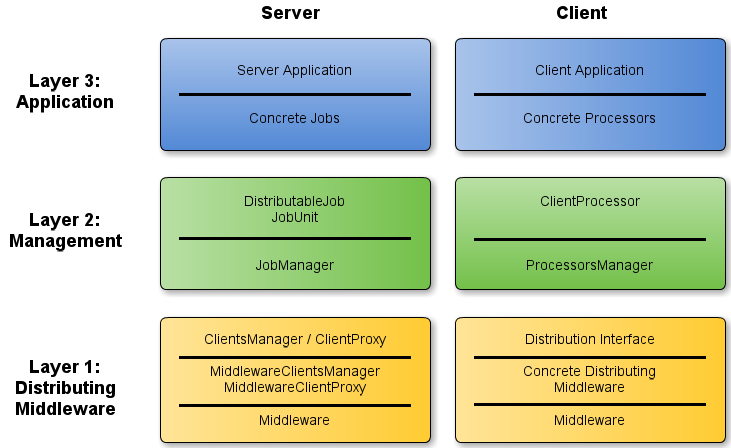
\includegraphics[scale=.4]{images/AbstractLayers-FuD.png}
	      \end{center}
	\end{frame}

	\begin{frame}\frametitle{Trabajos de FuD}
		\begin{block}{DistributableJob}
			Es un concepto de trabajo abstracto que encapsula cualquier tarea que será computada y puede ser subdividido en tareas más
			pequeñas llamadas \textbf{JobUnits}.
		\end{block}
		
		\pause
		\begin{block}{JobUnit}
			Representa una computación concreta y atómica que será llevada a cabo por alguno de los nodos de procesamiento. La tarea en 
			sí es representada por un mensaje el cual será pasado a un cliente de procesamiento quien se encargará de computarla.
		\end{block}
		
		\begin{center}
			%se pone asi para que \pause tenga efecto sobre la imagen
			\visible<2>{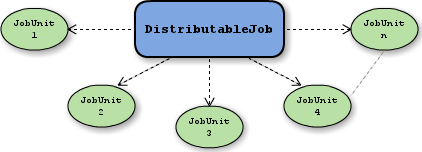
\includegraphics[scale=.4]{images/trabajos-fud.png}} 
		\end{center}
	\end{frame}
	
\end{subsection}

\begin{subsection}{Computación Voluntaria}

	\begin{frame}\frametitle{Computación Voluntaria}
		\begin{block}{Definición}
			La computación voluntaria es un tipo de computación distribuida donde personas (voluntarios) donan los recursos libres de 
			su ordenador a proyectos científicos mediante una conexión a internet.
		\end{block}
		
		\begin{center}
			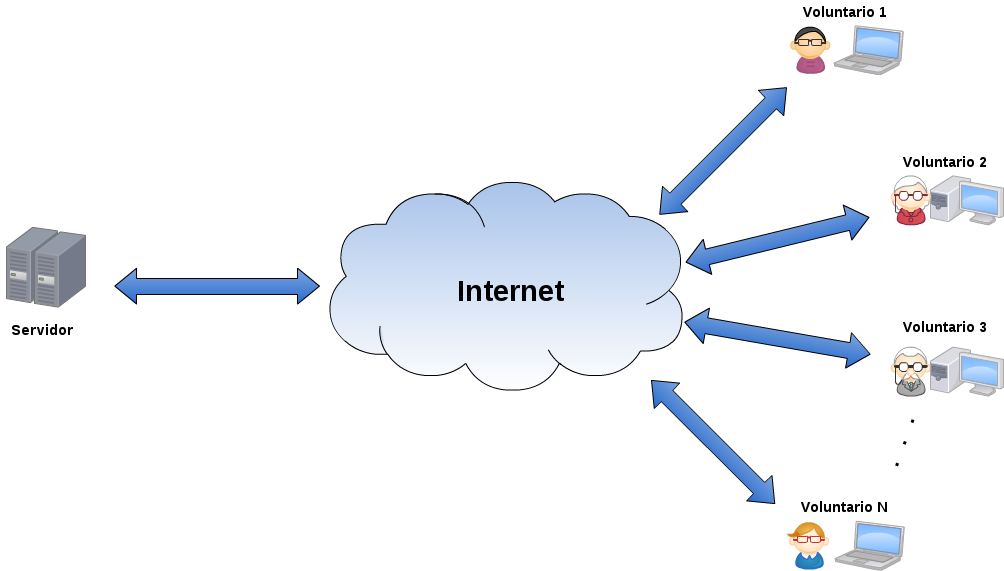
\includegraphics[scale=.22]{images/graf-comp-volunt.png}
		\end{center}
	\end{frame}

	\begin{frame}\frametitle{Computación Voluntaria}
		\textbf{Ventajas:\\[.5cm]}
		\begin{itemize}
			\addtolength{\itemsep}{3mm}
		    \item Los voluntarios pueden colaborar desde cualquier punto geográfico.
		    \item Hace posible la existencia de proyectos de investigación a bajos costos.
		    \item Los voluntarios no necesitan ser usuarios avanzados de computadoras.
		    \item Permite obtener y superar el poder de cálculo de una súper computadora.
		\end{itemize}
	\end{frame}

	\begin{frame}\frametitle{Computación Voluntaria}
		\textbf{Desventajas:\\[.5cm]}
		\begin{itemize}
		\addtolength{\itemsep}{3mm}
			\item Aumenta el consumo de energía de los ordenadores clientes debido a que éstos reducen su consumo en su tiempo libre.
			\item Para lograr un buen desempeño del proyecto es necesario apelar a medios de comunicación para reclutar voluntarios.
			\item Los voluntarios pueden confiar en los proyectos pero el proyecto no puede confiar en ellos.
		\end{itemize}
	\end{frame}
	
\end{subsection}

\begin{subsection}{BOINC}

	\begin{frame}\frametitle{Berkeley Open Infrastructure for Network Computing (BOINC)}
		\begin{block}{}
			\textbf{BOINC} es una plataforma de software de código abierto para computación voluntaria y computación grid, 
			cuyo principal propósito es hacer posible la investigación científica.
		\end{block}
		\pause
		\vspace{4mm}
		\textbf{Características}
		\begin{itemize}
			\item Los voluntarios pueden computar desde distintas plataformas.
			\item Los usuarios pueden participar en varios proyectos a la vez.
			\item Sólo se asignan tareas a voluntarios que cuenten con los recursos necesarios.
			\item Asignación de trabajos bajo demanda por parte de los clientes.
		\end{itemize}
	\end{frame}

	\begin{frame}\frametitle{Trabajos BOINC}
		Los trabajos de BOINC se encapsulan bajo dos conceptos importantes:
		\pause
		\vspace{4mm}
		\begin{block}{Workunit}
			Describe y representa la tarea a ser computada por un cliente del proyecto. Cada una está asociada a una aplicación en
			particular y puede tener uno o más archivos de entrada relacionados.
		\end{block}
		\pause
		\vspace{4mm}
		\begin{block}{Result}
			Es una instancia de una workunit que se desea resolver. Precisamente es este result el que será enviado a los clientes
			de BOINC para su procesamiento. Cada workunit debe tener asociado al menos un result.
		\end{block}
	\end{frame}

	\begin{frame}\frametitle{Proyecto BOINC}
		\begin{block}{}
			Un \textbf{proyecto BOINC} es el encargado de manegar todo el proceso de computación distribuida. Permite la 
			administración de cuentas de usuarios, de aplicaciones y define cómo van a ser distribuidos los trabajos.
		\end{block}
		\pause
		\vspace{2mm}
		\textbf{Componentes de un proyecto:}
		\begin{itemize}
			\item Una base de datos
			\item Un sitio web
			\item Un servidor conformado por:
			\begin{itemize}
				\item Generadores de trabajos \textit{(work generators)}
				\item Aplicaciones
				\item Utilidades \textit{(ej: start, stop, status, xadd, update\_version)}
				\item Demonios \textit{(ej: validator, assimilator, file\_deleter, db\_purge)}
			\end{itemize}
			\item Un archivo de configuración 
		\end{itemize}
		\vspace{2mm}
		\begin{block}{}
			Todo proyecto se identifica por la URL de su sitio web.
		\end{block}	
	\end{frame}
	
	\begin{frame}\frametitle{Proyectos conocidos}
		\begin{itemize}
		\addtolength{\itemsep}{2mm}
			\item Seti@home\\ (\url{http://setiathome.ssl.berkeley.edu/})
			\item Climate Prediction\\ (\url{http://climateprediction.net/})
			\item LHC@Home\\ (\url{http://lhcathomeclassic.cern.ch/sixtrack/})
			\item Einstein@Home\\ (\url{http://einstein.phys.uwm.edu/})			
		\end{itemize}
		\vspace{6mm}
		Lista completa de proyectos BOINC:\\
		\url{http://boinc.berkeley.edu/wiki/Project_list/}
	\end{frame}
	

	\begin{frame}\frametitle{Cliente BOINC y BOINC Manager}
		\begin{block}{Cliente BOINC \texttt{(core client)}}
			Es la aplicación cliente de BOINC que corre como demonio en las computadoras de los participantes.
		\end{block}	
		\pause
		\textbf{Sus principales funciones son:}
		\begin{itemize}
			\item Mantener una conexión directa con el servidor del proyecto para recibir trabajos y enviar resultados.
			\item Descargar la aplicación necesaria para la computación de cada trabajo.
			\item Realizar la computación de cada tarea.
			\item Administrar la distribución de los recursos locales entre los proyectos adheridos.
		\end{itemize}
		\pause
		\vspace{2mm}
		\begin{block}{BOINC Manager}
			Es una aplicación que ofrece una simple interfaz gráfica mediante la cuál los voluntarios pueden controlar el 
			\textbf{cliente BOINC}.
		\end{block}	
	\end{frame}

	\begin{frame}\frametitle{Componentes de BOINC}
		\begin{center}
			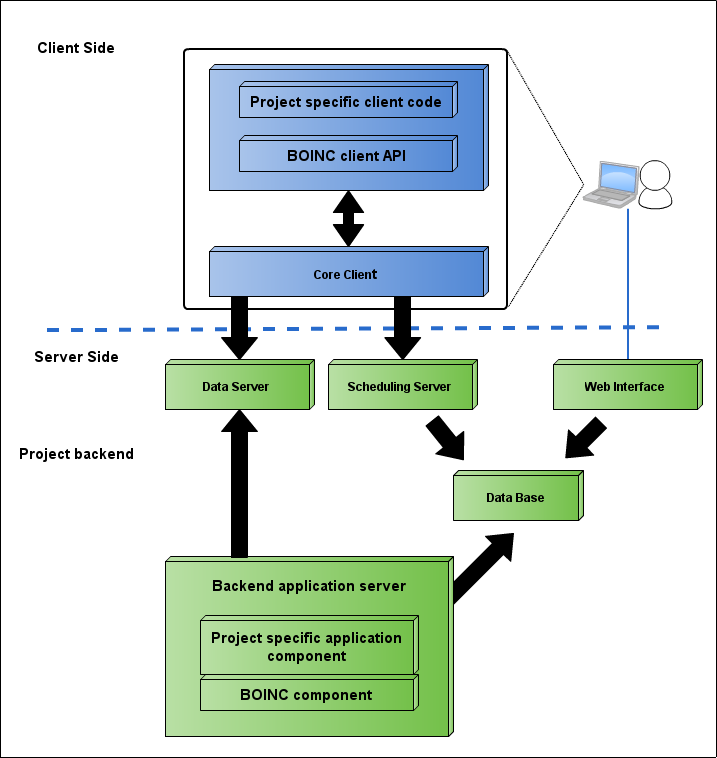
\includegraphics[scale=0.25]{images/componentes-boinc.png}
		\end{center}
	\end{frame}

	\begin{frame}\frametitle{Interacción entre servidor y cliente BOINC}
		\begin{center}
			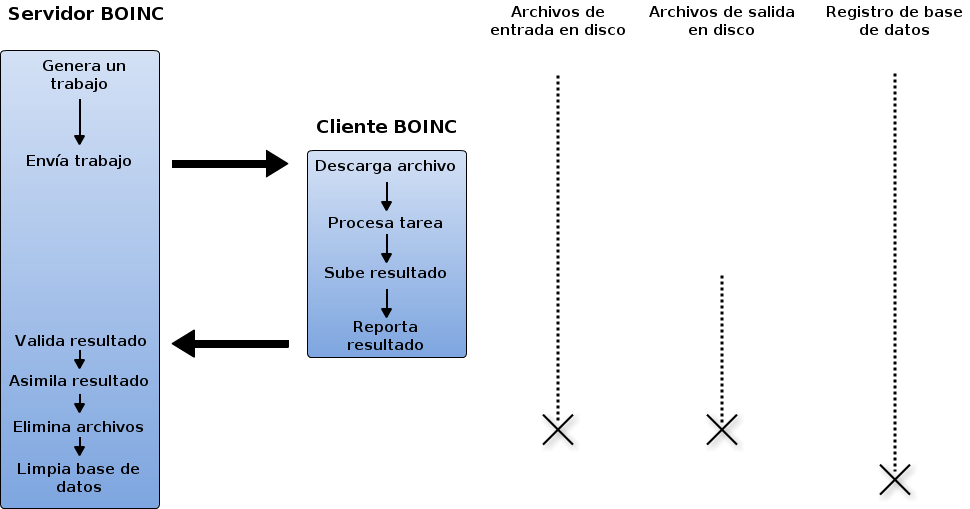
\includegraphics[scale=0.32]{images/Client-Server-Interact.png}
		\end{center}
	\end{frame}
	
\end{subsection}
